\documentclass[]{article}

% include packages needed for your report
\usepackage{graphicx, verbatim} % to include figures
\usepackage{caption,subcaption} % to include captions and sub captions to figures
\usepackage{titling} % to format title page
\renewcommand\maketitlehooka{\null\mbox{}\vfill} % to center title page
\renewcommand\maketitlehookd{\vfill\null}
\usepackage[margin=1.1in]{geometry} % to adjust the page margin
\usepackage{amsmath} % to display equations
\usepackage{csquotes} % to quote
\usepackage{float} % specify figure and table location
\usepackage{fancyhdr} % to add header
\usepackage{lastpage} % to put the current page number in context of page numbers in the whole document
\usepackage[nottoc,numbib]{tocbibind} % to give section number for the reference
\usepackage{enumitem} % to adjust spacing between bullet point and dashed line
\usepackage{longtable}

\pagestyle{fancy}
\fancyhf{}
\cfoot{Page \thepage \hspace{0.9pt} of \pageref{LastPage}}

\rhead{M6A}
\lhead{
\includegraphics[scale=0.02]{uclalogo.png}}

\title{\Huge Prostate Cancer Active Surveillance }
\date{\today}
\author{\\[1cm]
      Author Alfonso Lam\\[1.5cm]
      Boutros Lab\\
      Jonsson Comprehensive Cancer Center\\
      }

% begin report
\begin{document}

% title page
\begin{titlingpage}
\maketitle
\begin{figure}
    \centering
    
\includegraphics[scale=0.03]{uclalogo.png}
    \label{fig:my_label}
\end{figure}
\end{titlingpage}

% The idea here is that patients with prostate cancer often go on
% something called “Active Surveillance” (AS). This means that they
% have the disease, but the chance of it becoming aggressive and moving
% outside of the prostate is very low (~5-10%).
%
% Because this chance is low, patients will often be “surveilled” to
% see if their disease advances
% using a combination of blood tests, imaging and biopsies. The current
% prediction of “is this cancer aggressive” is not perfect, and in
% fact biopsy is an aggressive & expensive procedure.  There is therefore
% a need to do a better job in making these predictions.
% 
% Our colleague in San Antonio, Dr. Michael Liss, is a prostate cancer
% surgeon (i.e. a urologist) and has accumulated a cohort of 123 patients
% who were on AS a fraction of which went on to aggressive disease
% (the “Biopsy Upgraded” column in the
% MRI DOD Biomarkers Database_Boutros – 2019.11.12.xlsx).
% He then did a series of imaging, genetic, blood and urine tests on
% these patients to try to predict aggressive disease.
% 
% The questions we have in this dataset are two-fold:
% 
% 1.- What features best predict aggressive disease?
% 
% 2.- In what order (sequence) should different biomarkers be run
% to maximize sensitivity and specificity, while minimizing cost?
% Note here that the word “sequence” in this study can both refer to the
% technology used to analyze genetic information on patients
% (“they were sequenced” or “sequencing data”) and to the ordering of different
% tests (“what sequence should these tests be run?”) and it will be critical
% that you are extremely clear in writing which of these two you’re
% referring to at all times.
% 
% As you’ll see there are a couple of files labeled –Key which explain
% the individual features.  As with the m6A-writer dataset you will want
% to start with exploratory analysis (EDA – exploratory data analysis):
% 
% Look at distributions
% Look at correlations amongst variables
% Create some plots outlining the dataset as a whole
% 
% Then you’ll move on to univariate analyses
% 
% How does each predictive feature correlate to the outcome variable?
% 
% Then you’ll move on to sequencing of biomarkers.
% This will involve considering all the biomarkers that emerge from a
% single assay and asking which assay provides the most information
% as an initial test, and then which is most complementary to it, and so forth.
% We will then likely consider the “cost” (financial) of each biomarker
% as a weight in this decision making, but we can consider detailed
% strategies at a later date once we’ve seen the EDA.
% 
% As before, I want this sequentially built up into a PDF report in
% the lab format, so that at any point in time we have a report of all
% the results that have been generated to date, along with their associated
% methods.  And I’ll link you in a moment to Dr. Liss, although let me
% know before you ask him any questions directly as he’s a surgeon and
% I don’t want to take up his time with minor questions.

% report outline
\section{Introduction}

\subsection{Study Design and Objectives}
\noindent In this study, a group of individuals with prostate cancer is on 
“Active Surveillance” (AS). AS is a combination of blood tests, imaging and biopsies. 
It intends to monitor the progression of the disease, but the current prediction of 
the aggressiveness of prostate cancer is not perfect and need improvement. What features 
do the best job in predicting aggressive disease? In what order (sequence) should 
different biomarkers be run to maximize sensitivity and specificity, while minimizing cost?  

\subsection{Data Description}

\begin{center}
\begin{tabular}{ |c|p{2cm}|p{2cm}|}
\hline
  {\bf Filename} &  {\bf Number of Individuals} & {\bf Number of Columns}  \\
\hline
    MRI\_DOD\_Biomarkers\_Database\_Boutros$-$2020.04.20.xlsx &  123  & 53  \\
\hline
\end{tabular}
\end{center}

\section{Exploratory Data Analysis}

\noindent Some basic information from the individuals are available in the original dataset. 
We can start classifying the data by race (1=White, 2=African American, and 3=Asian-American 
or Pacific Islander). Figure~\ref{fig:basic} shows an idea of some of the basic features the 
patients have. The majority of the patients are white individuals. \\

\begin{figure}[H]
\centering
\begin{tabular}{|c|c|}
      \hline
      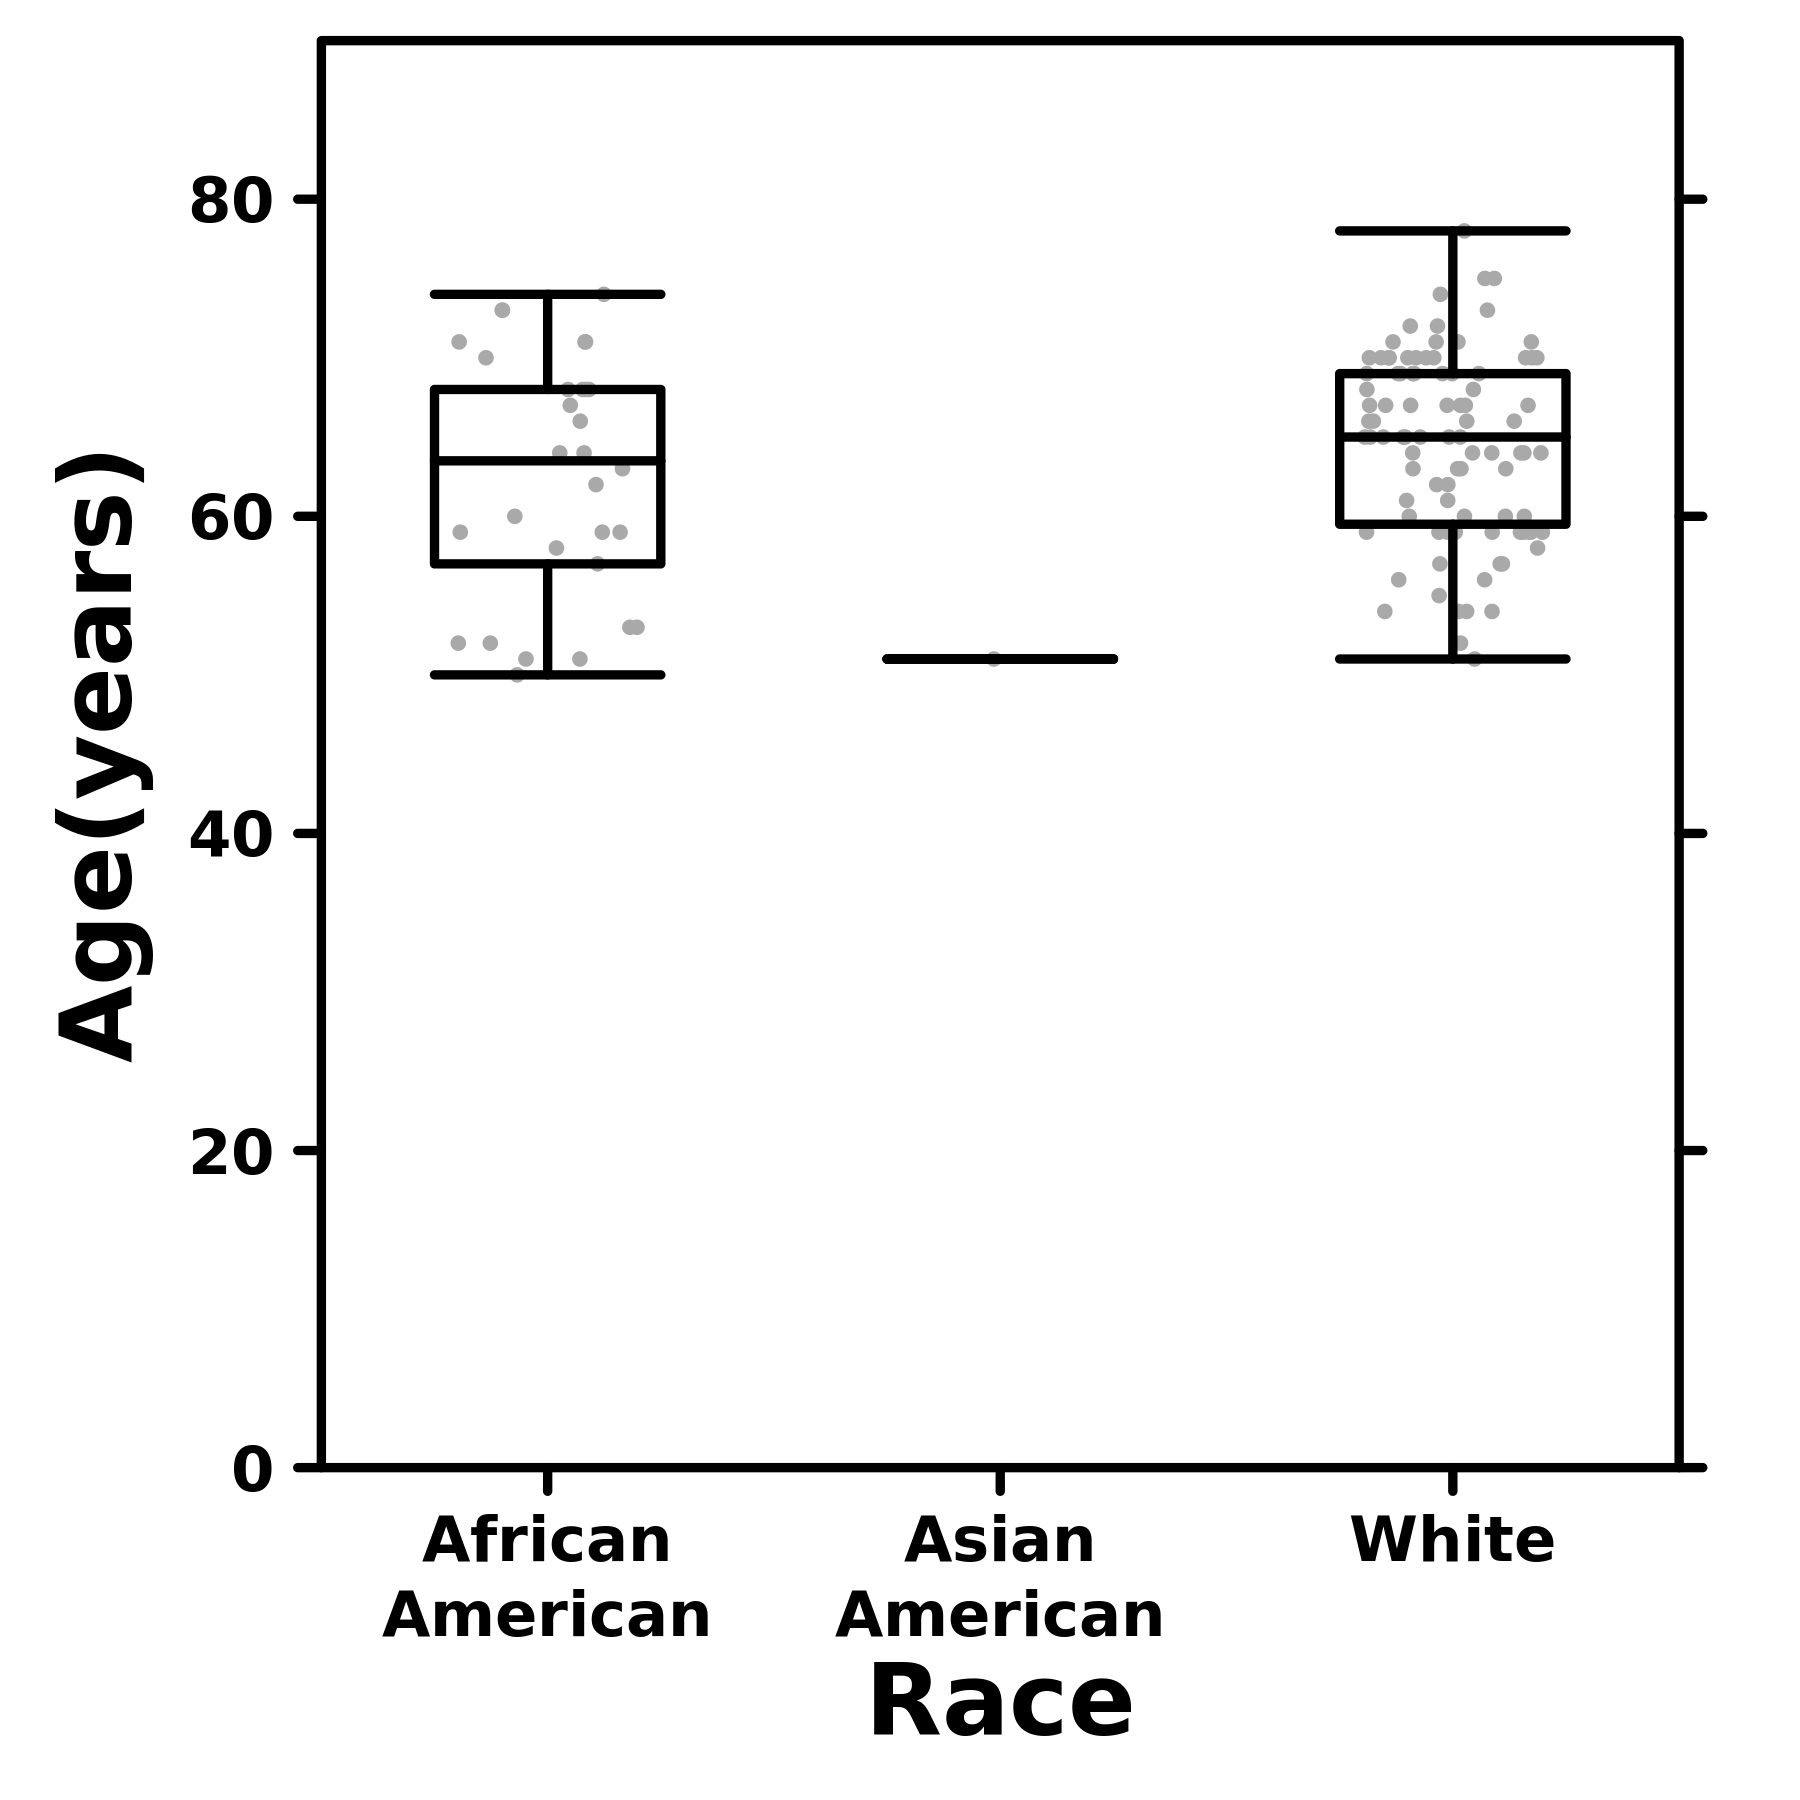
\includegraphics[width=50mm]{png/age.png} &
      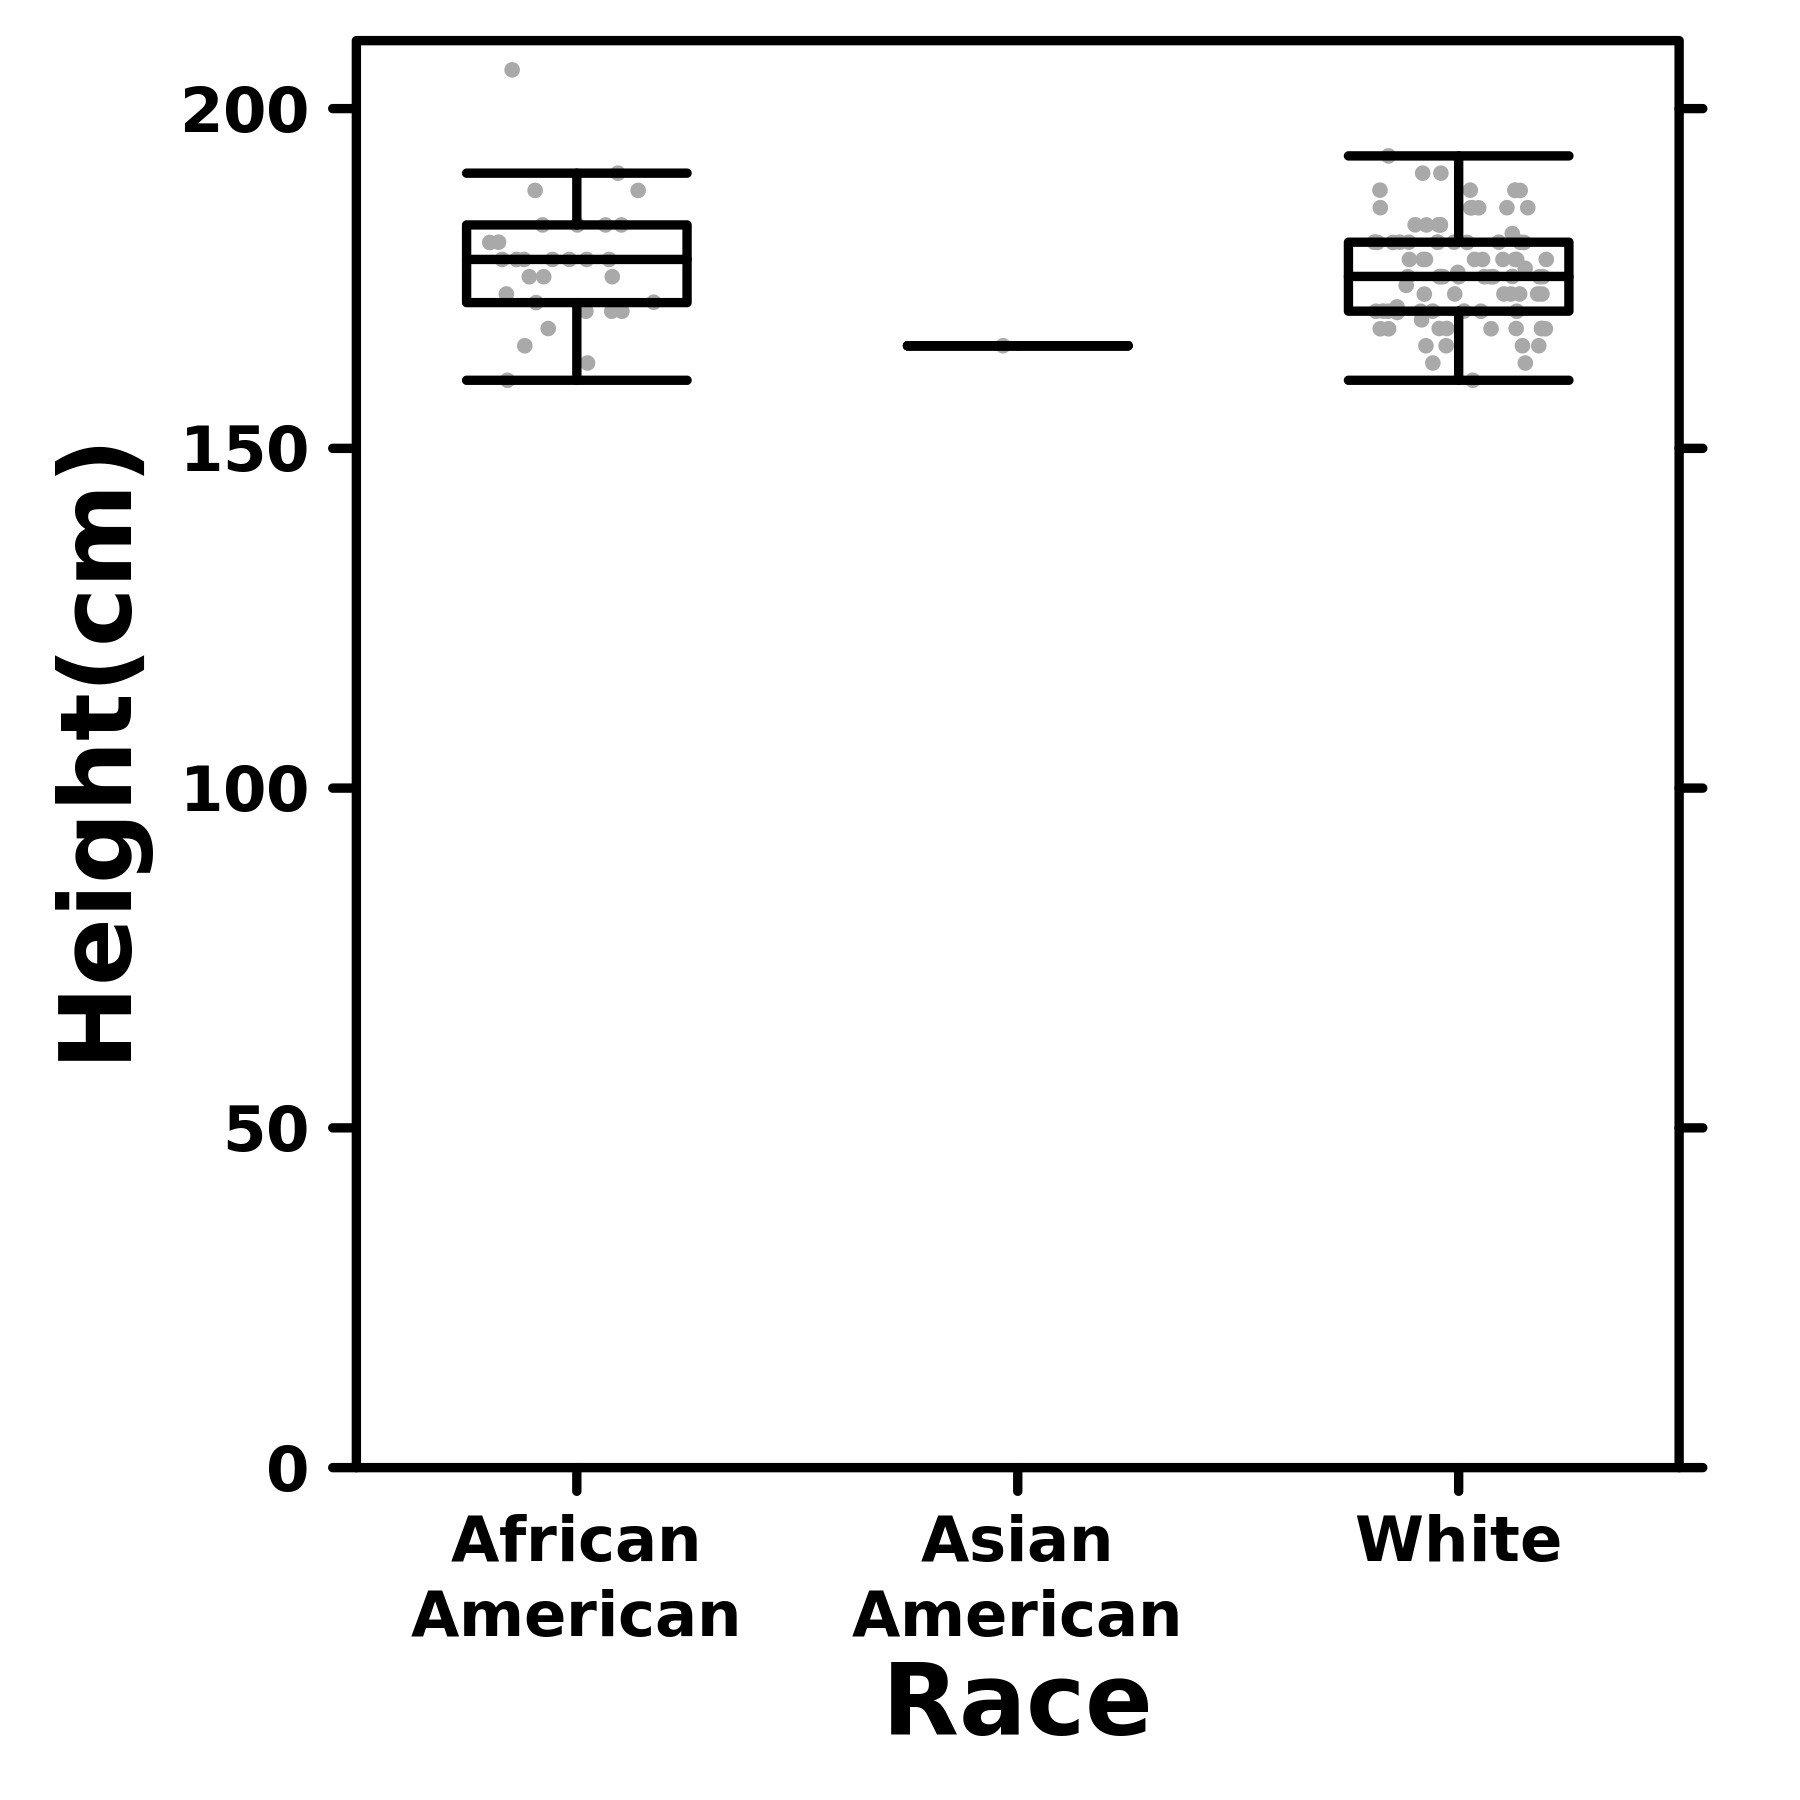
\includegraphics[width=50mm]{png/height.png} \\
      \hline
      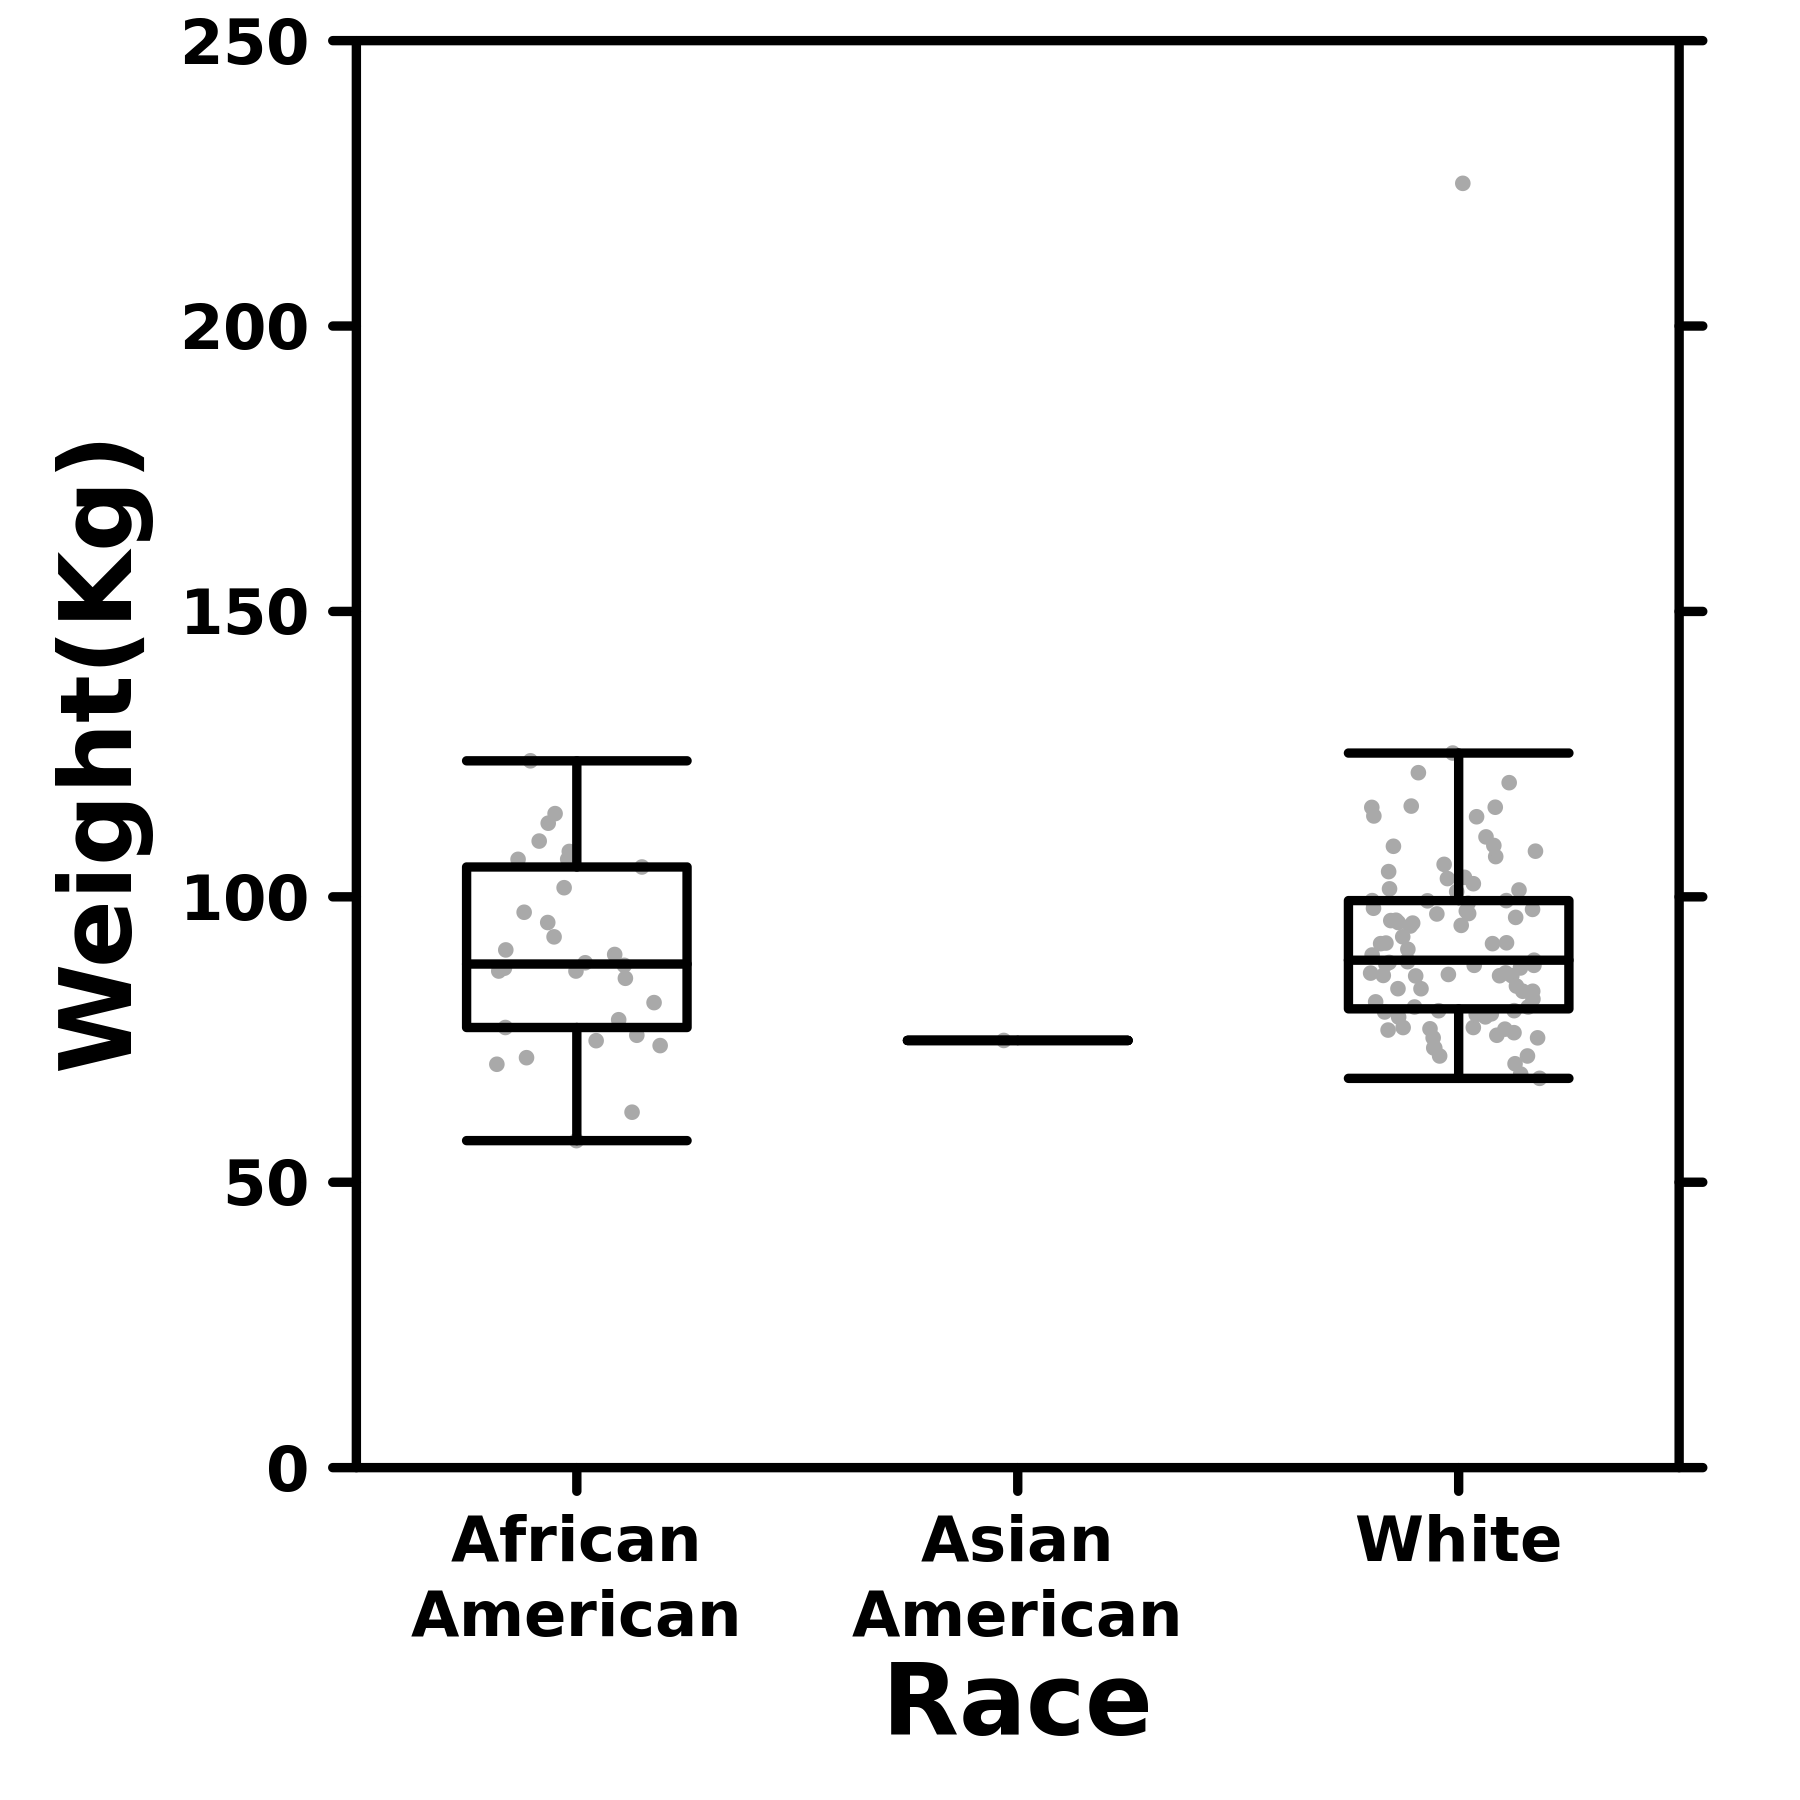
\includegraphics[width=50mm]{png/weight.png} & 
      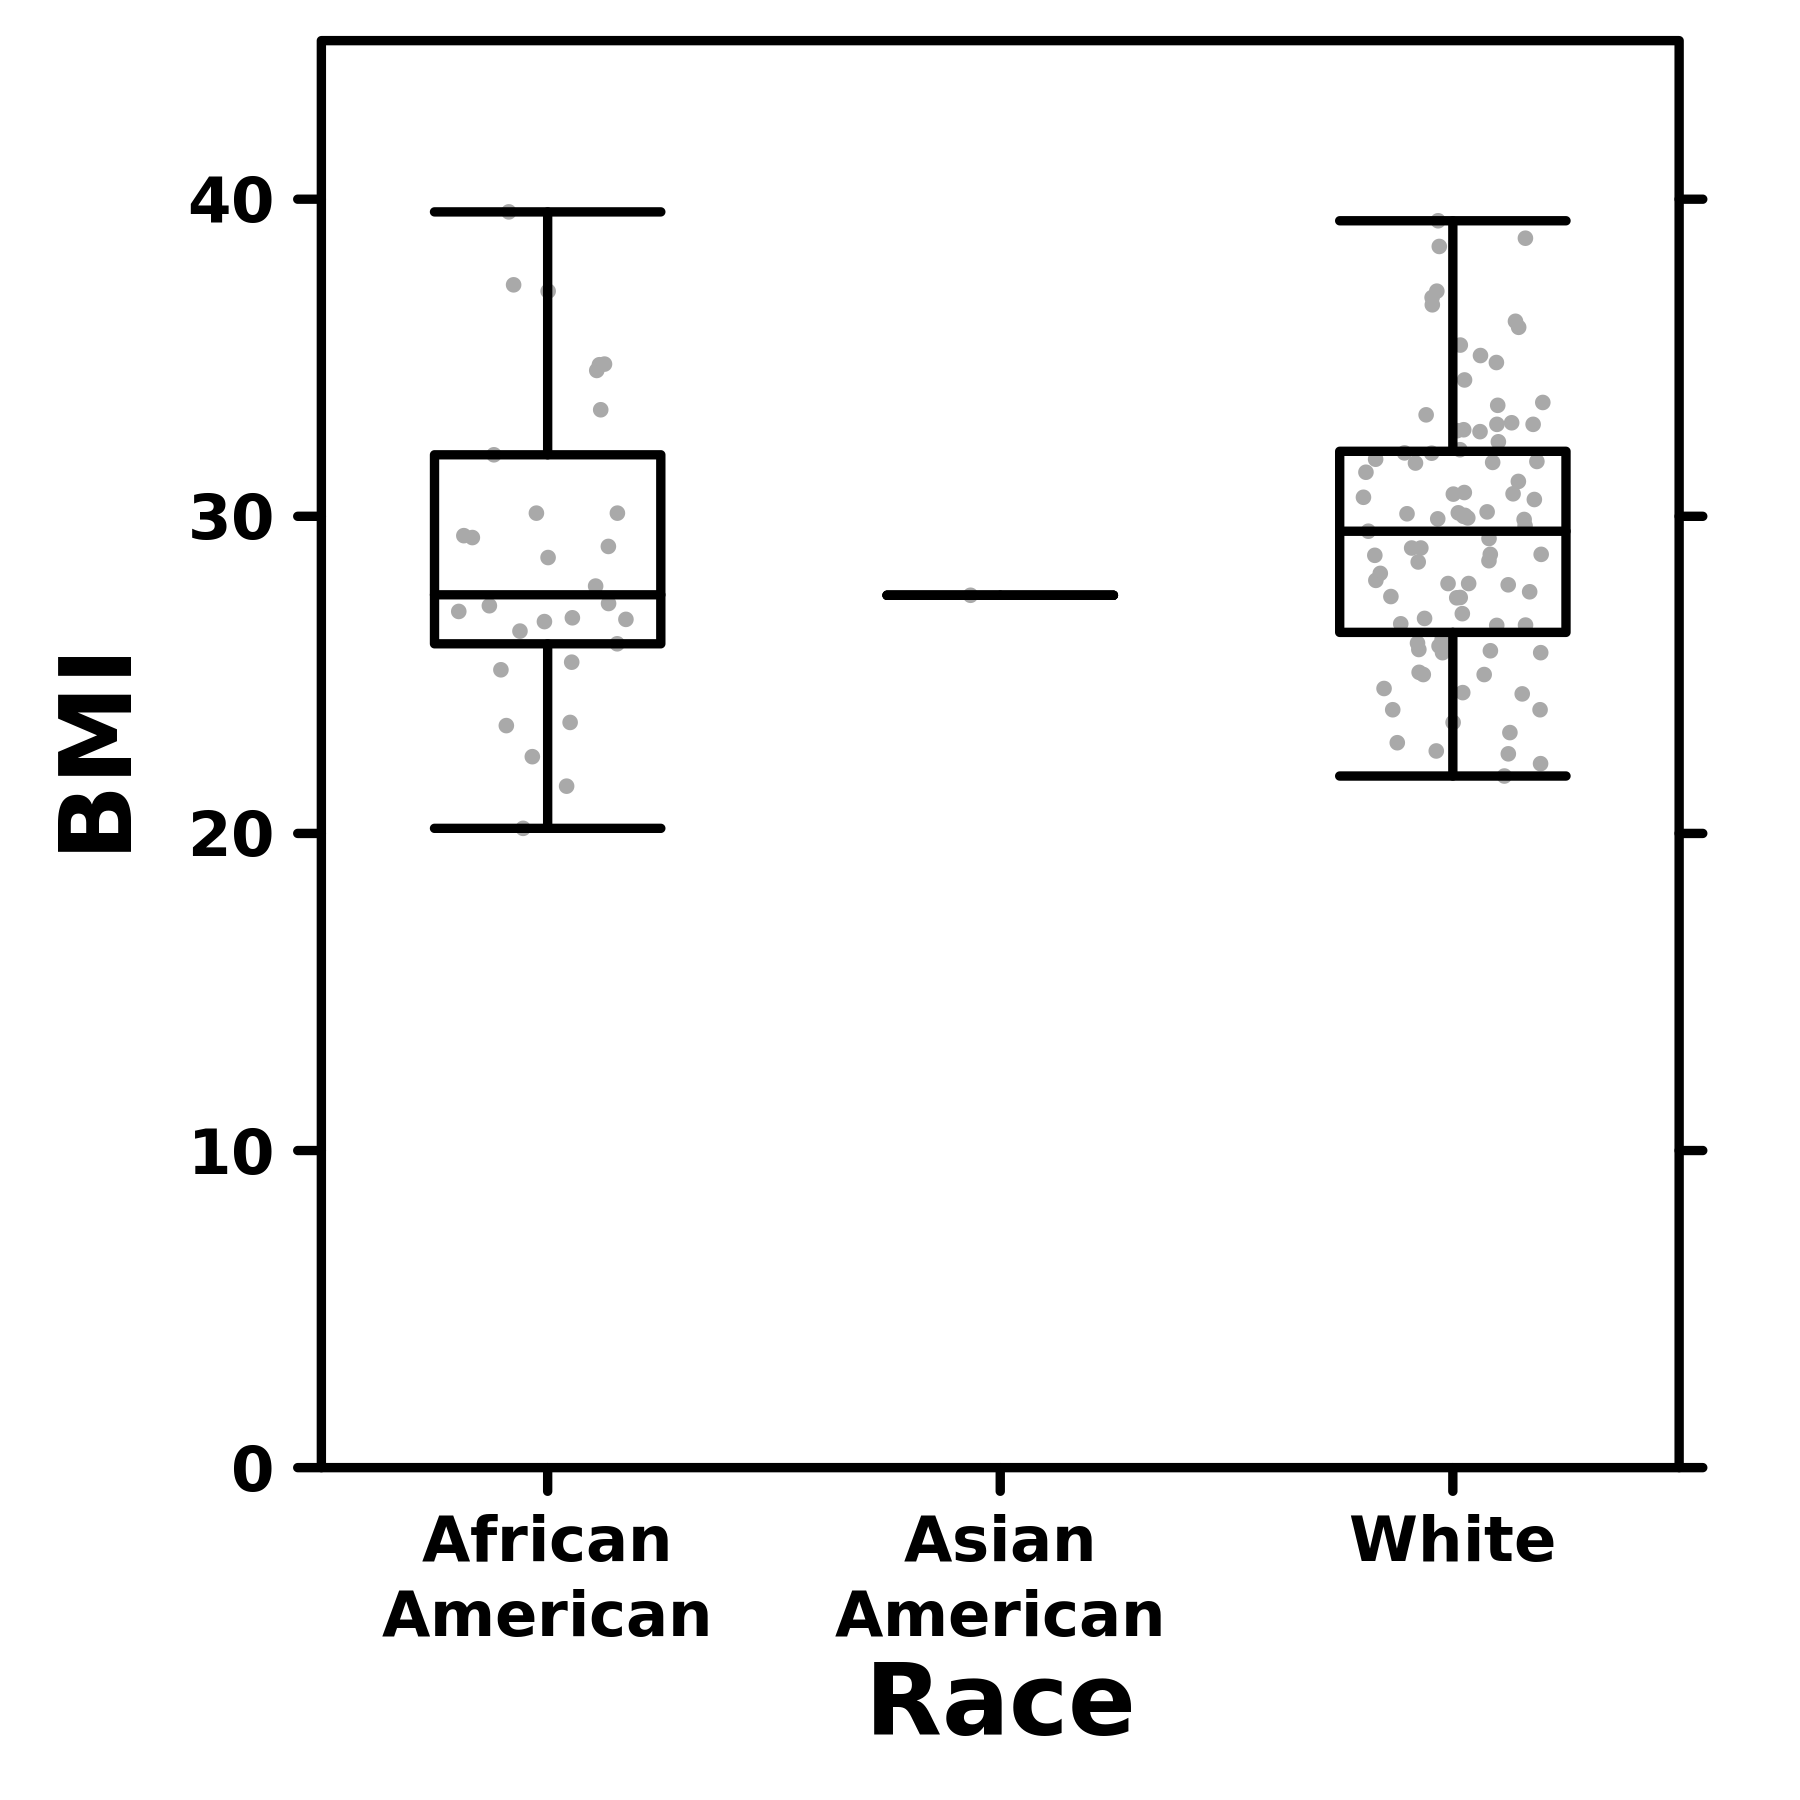
\includegraphics[width=50mm]{png/bmi.png} \\
      \hline
\end{tabular}
\caption{Basic information from individuals grouped by race: Afro-Am (African-American), Asian-Am
(Asian-American), and White}
\label{fig:basic}
\end{figure}

\noindent Figure~\ref{fig:basic2} shows the prostate volume distributed in the individuals. These individuals 
are patients that were administered blood test, urine test, MRI, biopsies, etc. They are currently in 
Active Survellaince (AS). We should keep in mind that not all of them completed.  \\

\begin{figure}
\centering
    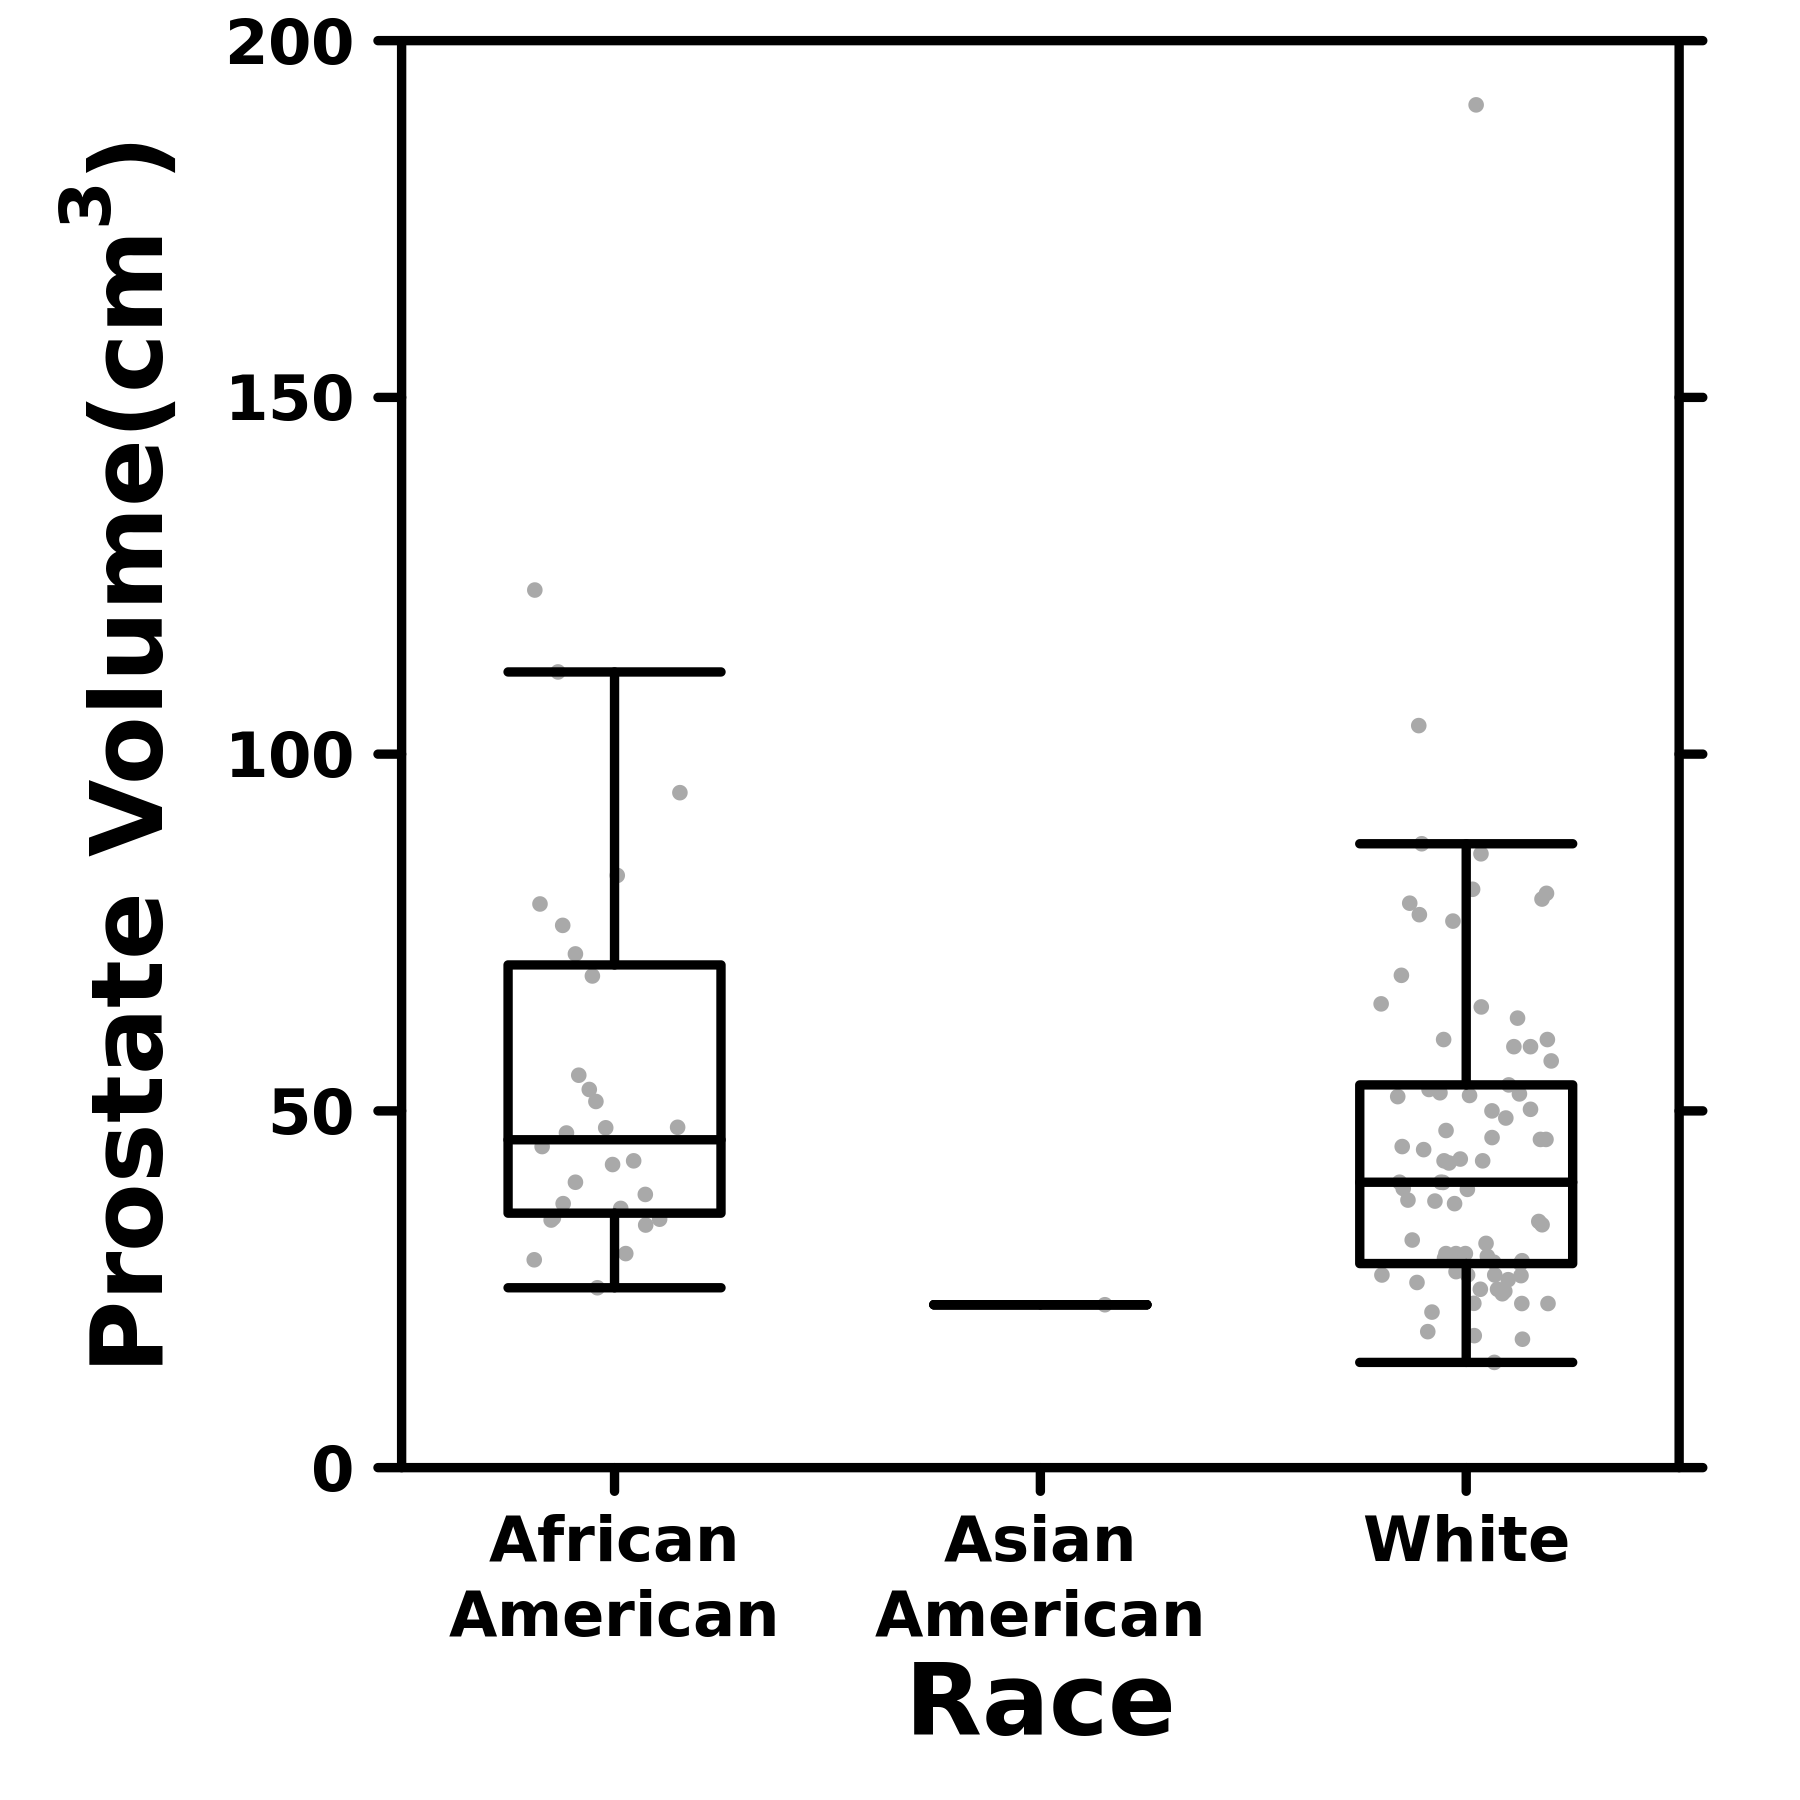
\includegraphics[width=60mm]{png/prostate_volume.png} \\
\caption{}
\label{fig:basic2}
\end{figure}

\noindent In the original dataset, most of those tests report numerical quantities or scores, and others  
reporting binary answers (0 or 1, etc). Some of those tests reporting scores have similatities with 
other tests in the list. We can take those tests and the features, and compute the correlation between them. 
Figure~\ref{fig:correlations} shows a heatmap of the correlations  where some tests are clearly correlated. 
That can help us to build our model and reduce some of the predictors. \\

\begin{figure}
\centering
    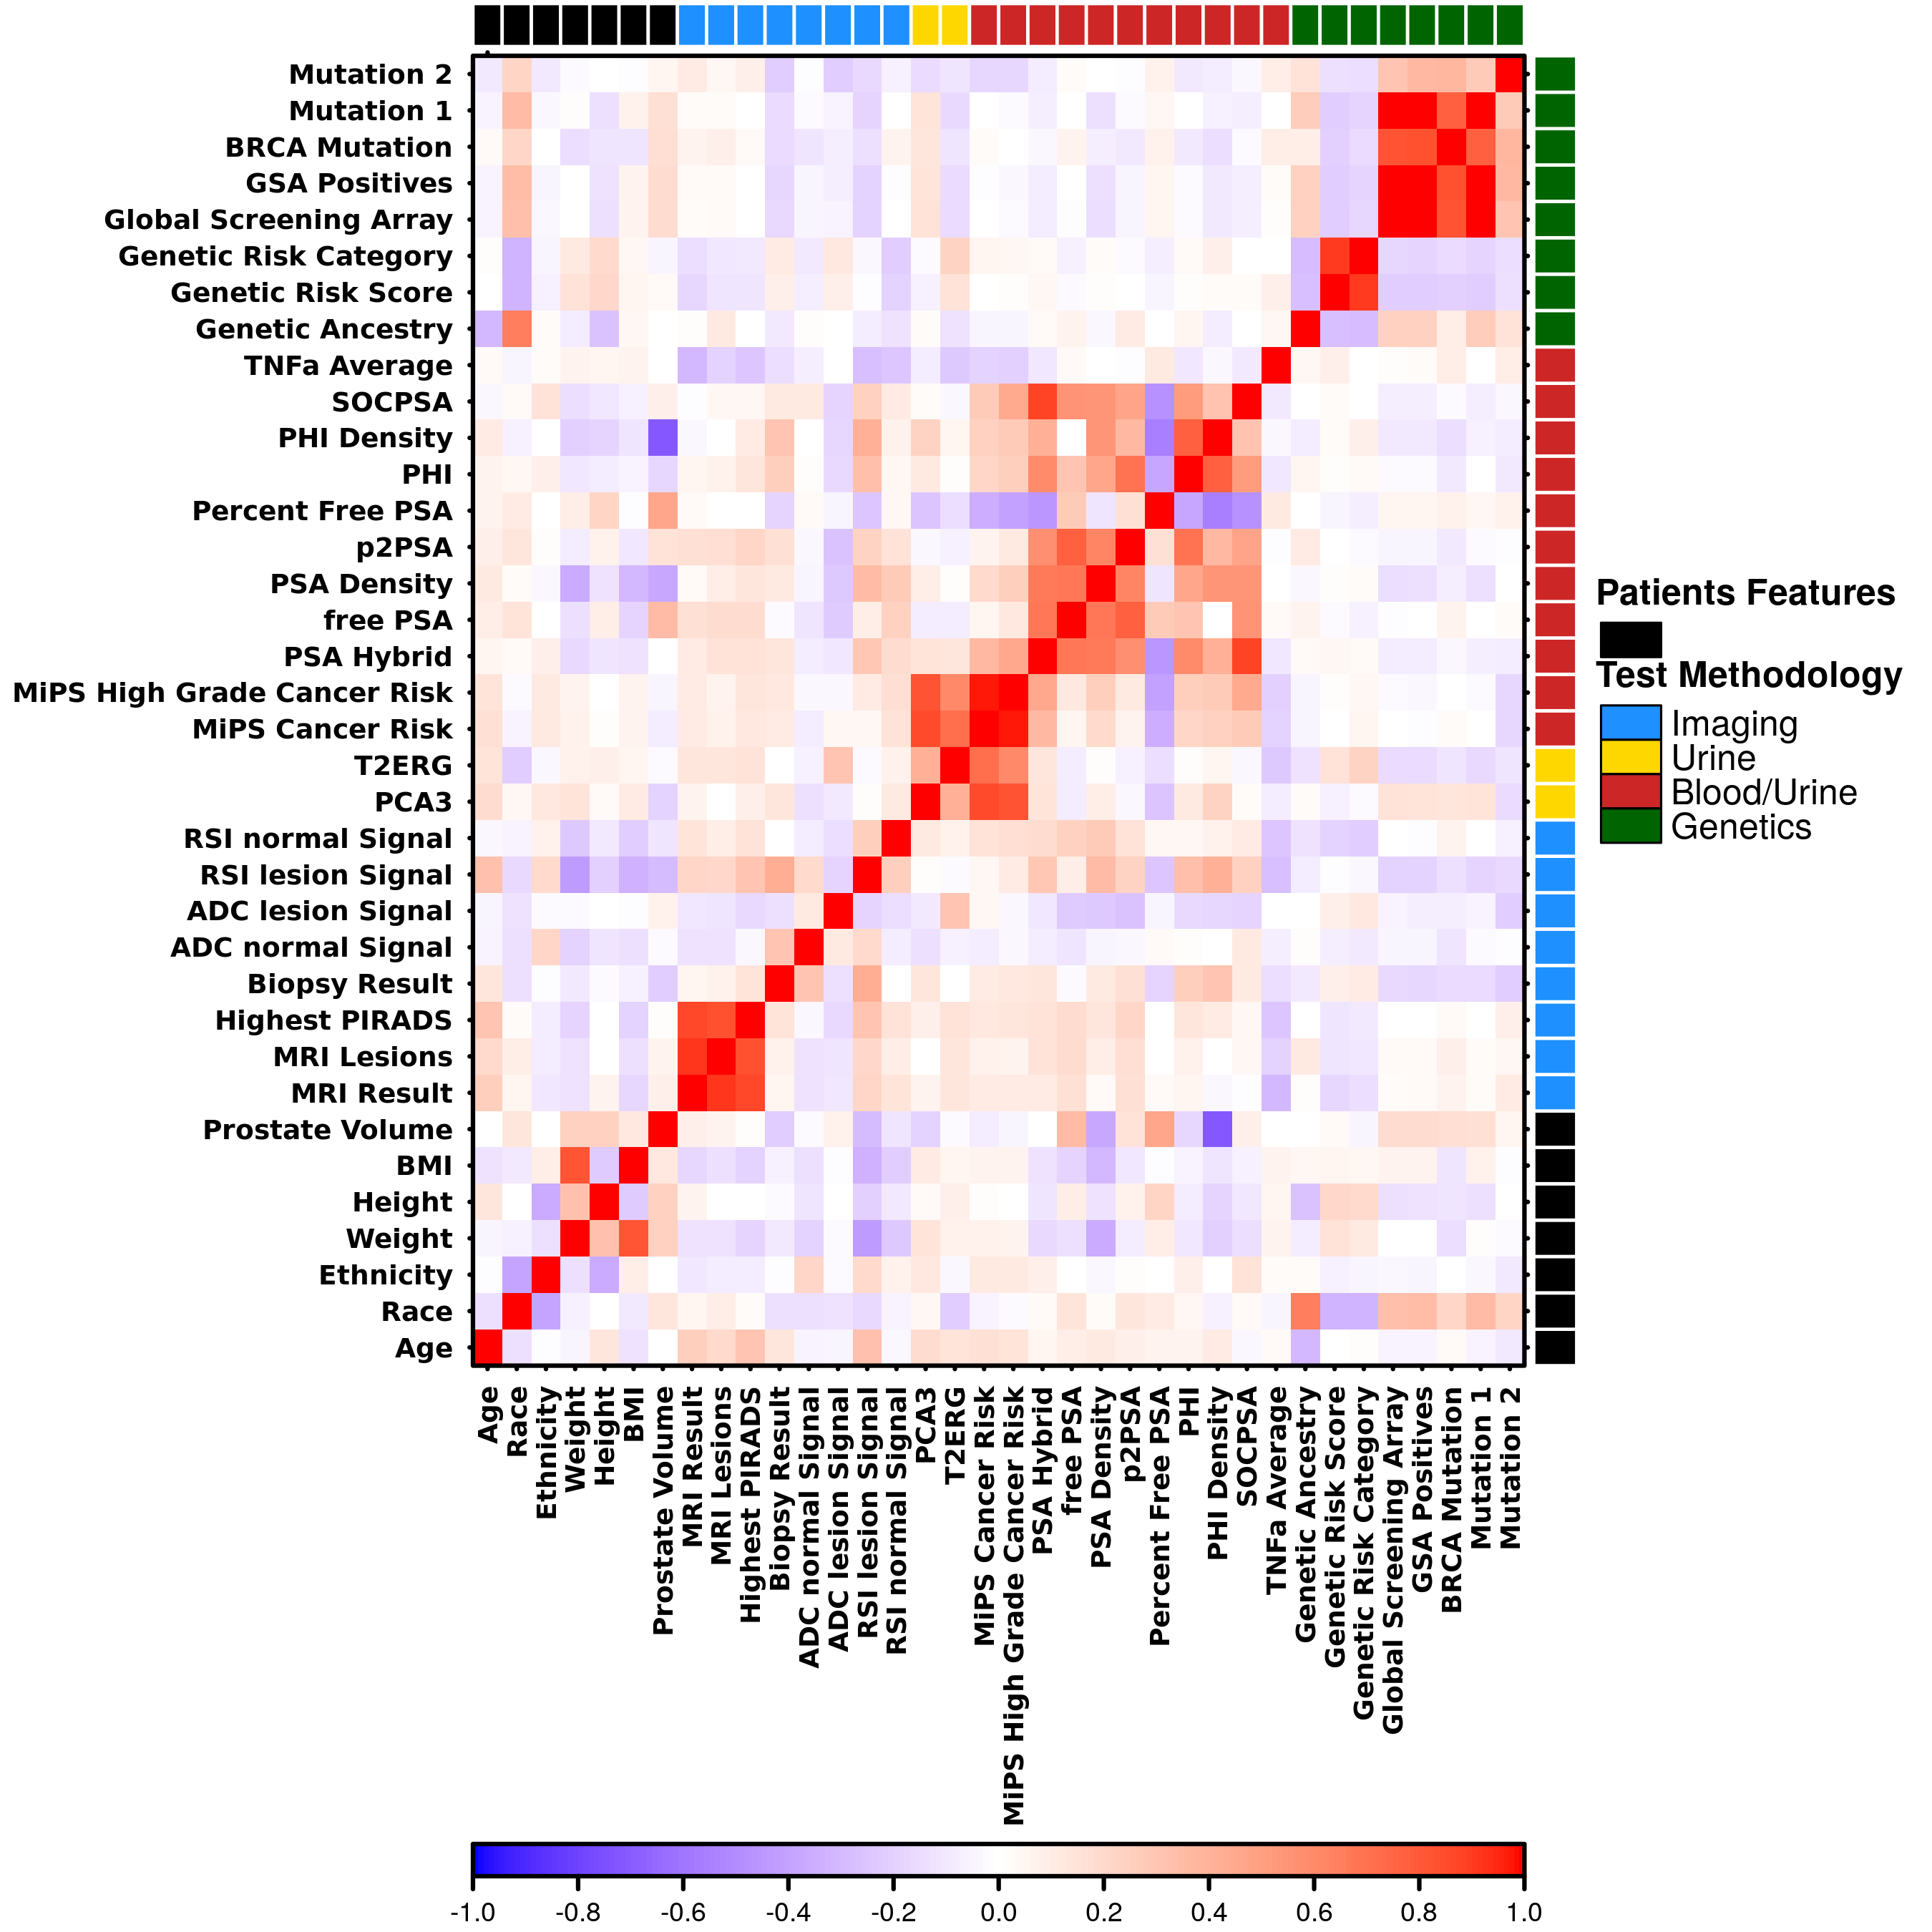
\includegraphics[width=100mm]{png/correlations.png} \\
\caption{Correlations between some tests performed in patients.}
\label{fig:correlations}
\end{figure}

\noindent By definition, a patient in AS has prostate cancer. Thus, a sequence of tests are performed during the
AS in order to monitor the progression of the disease. At some point in time, the doctor update the Biopsy information
({\verb|BiopsyUpgraded|}). It is a categorical variable (0=No, 1=Yes). We can attempt to find a relation between the 
{\verb|BiopsyUpgraded|} with the different biomarkers used in the AS. Those biomarkers are shown in 
table~\ref{tab:table1}. \\

\begin{center}
\begin{tabular}{|c|c|}
\hline
{\bf Category} & {\bf Biomarker}  \\
\hline
Urine  & PCA3  \\
\hline
Urine  & T2ERG  \\
\hline 
Blood/Urine &  MiPSCancerRisk  \\
\hline
Blood/Urine &  MiPSHighGradeCancerRisk  \\
\hline
Blood & PSAHyb  \\
\hline 
Blood & freePSA  \\
\hline
Blood & p2PSA \\
\hline
Blood & PercentFreePSA  \\
\hline
Blood & PHI \\
\hline
Genetics & GeneticAncestry  \\
\hline
Genetics & GeneticRiskScore  \\
\hline
Genetics & GeneticRiskCategory  \\
\hline
Genetics & GlobalScreeningArray  \\
\hline
Genetics & GSA Gene  \\
\hline
Imaging  & RSInormalSignal   \\
\hline
Imaging  & RSIlesionSignal  \\
\hline
Imaging  & ADCnormalSignal  \\
\hline
Imaging  & ADClesionSignal  \\
\hline
\end{tabular}
\label{tab:table1}
\end{center}

\noindent For each test, we evaluate its performance by plotting the Precision-Recall (PR) Curve. Recall or Sensitivity 
is the ability of the test to correctly mark all positive responses as positive. Precision is 
the ability of the test not to wrongly label a negative sample as positive.  To make the PR curve, 
we take the values of the test provided in the original data and consider the data from \verb|BiopsyUpgraded| as the response. 
Some tests were not taking into consideration here since there are categorical data. We use a set of thresholds to build the 
confusion matrix. The first threshold is the lowest value reported by the test. Above that threshold, all values are set to 
1, otherwise 0. The result is compared to the values from \verb|BiopsyUpgraded| and then the
confusion matrix is built. From that matrix, the true positive, true negative, false positiv, and false negative are determined.
Other variables such as accuracy, precision, sensitivity and specificity can be computed quickly from that matrix. This will be 
helpful to set a proper threshold to get the most benefits from the test. The AUPRC plots for all the tests shown in 
table~\ref{tab:table1} are displayed in Figure~\ref{fig:PRcurve}. \\

\begin{figure}
\centering
    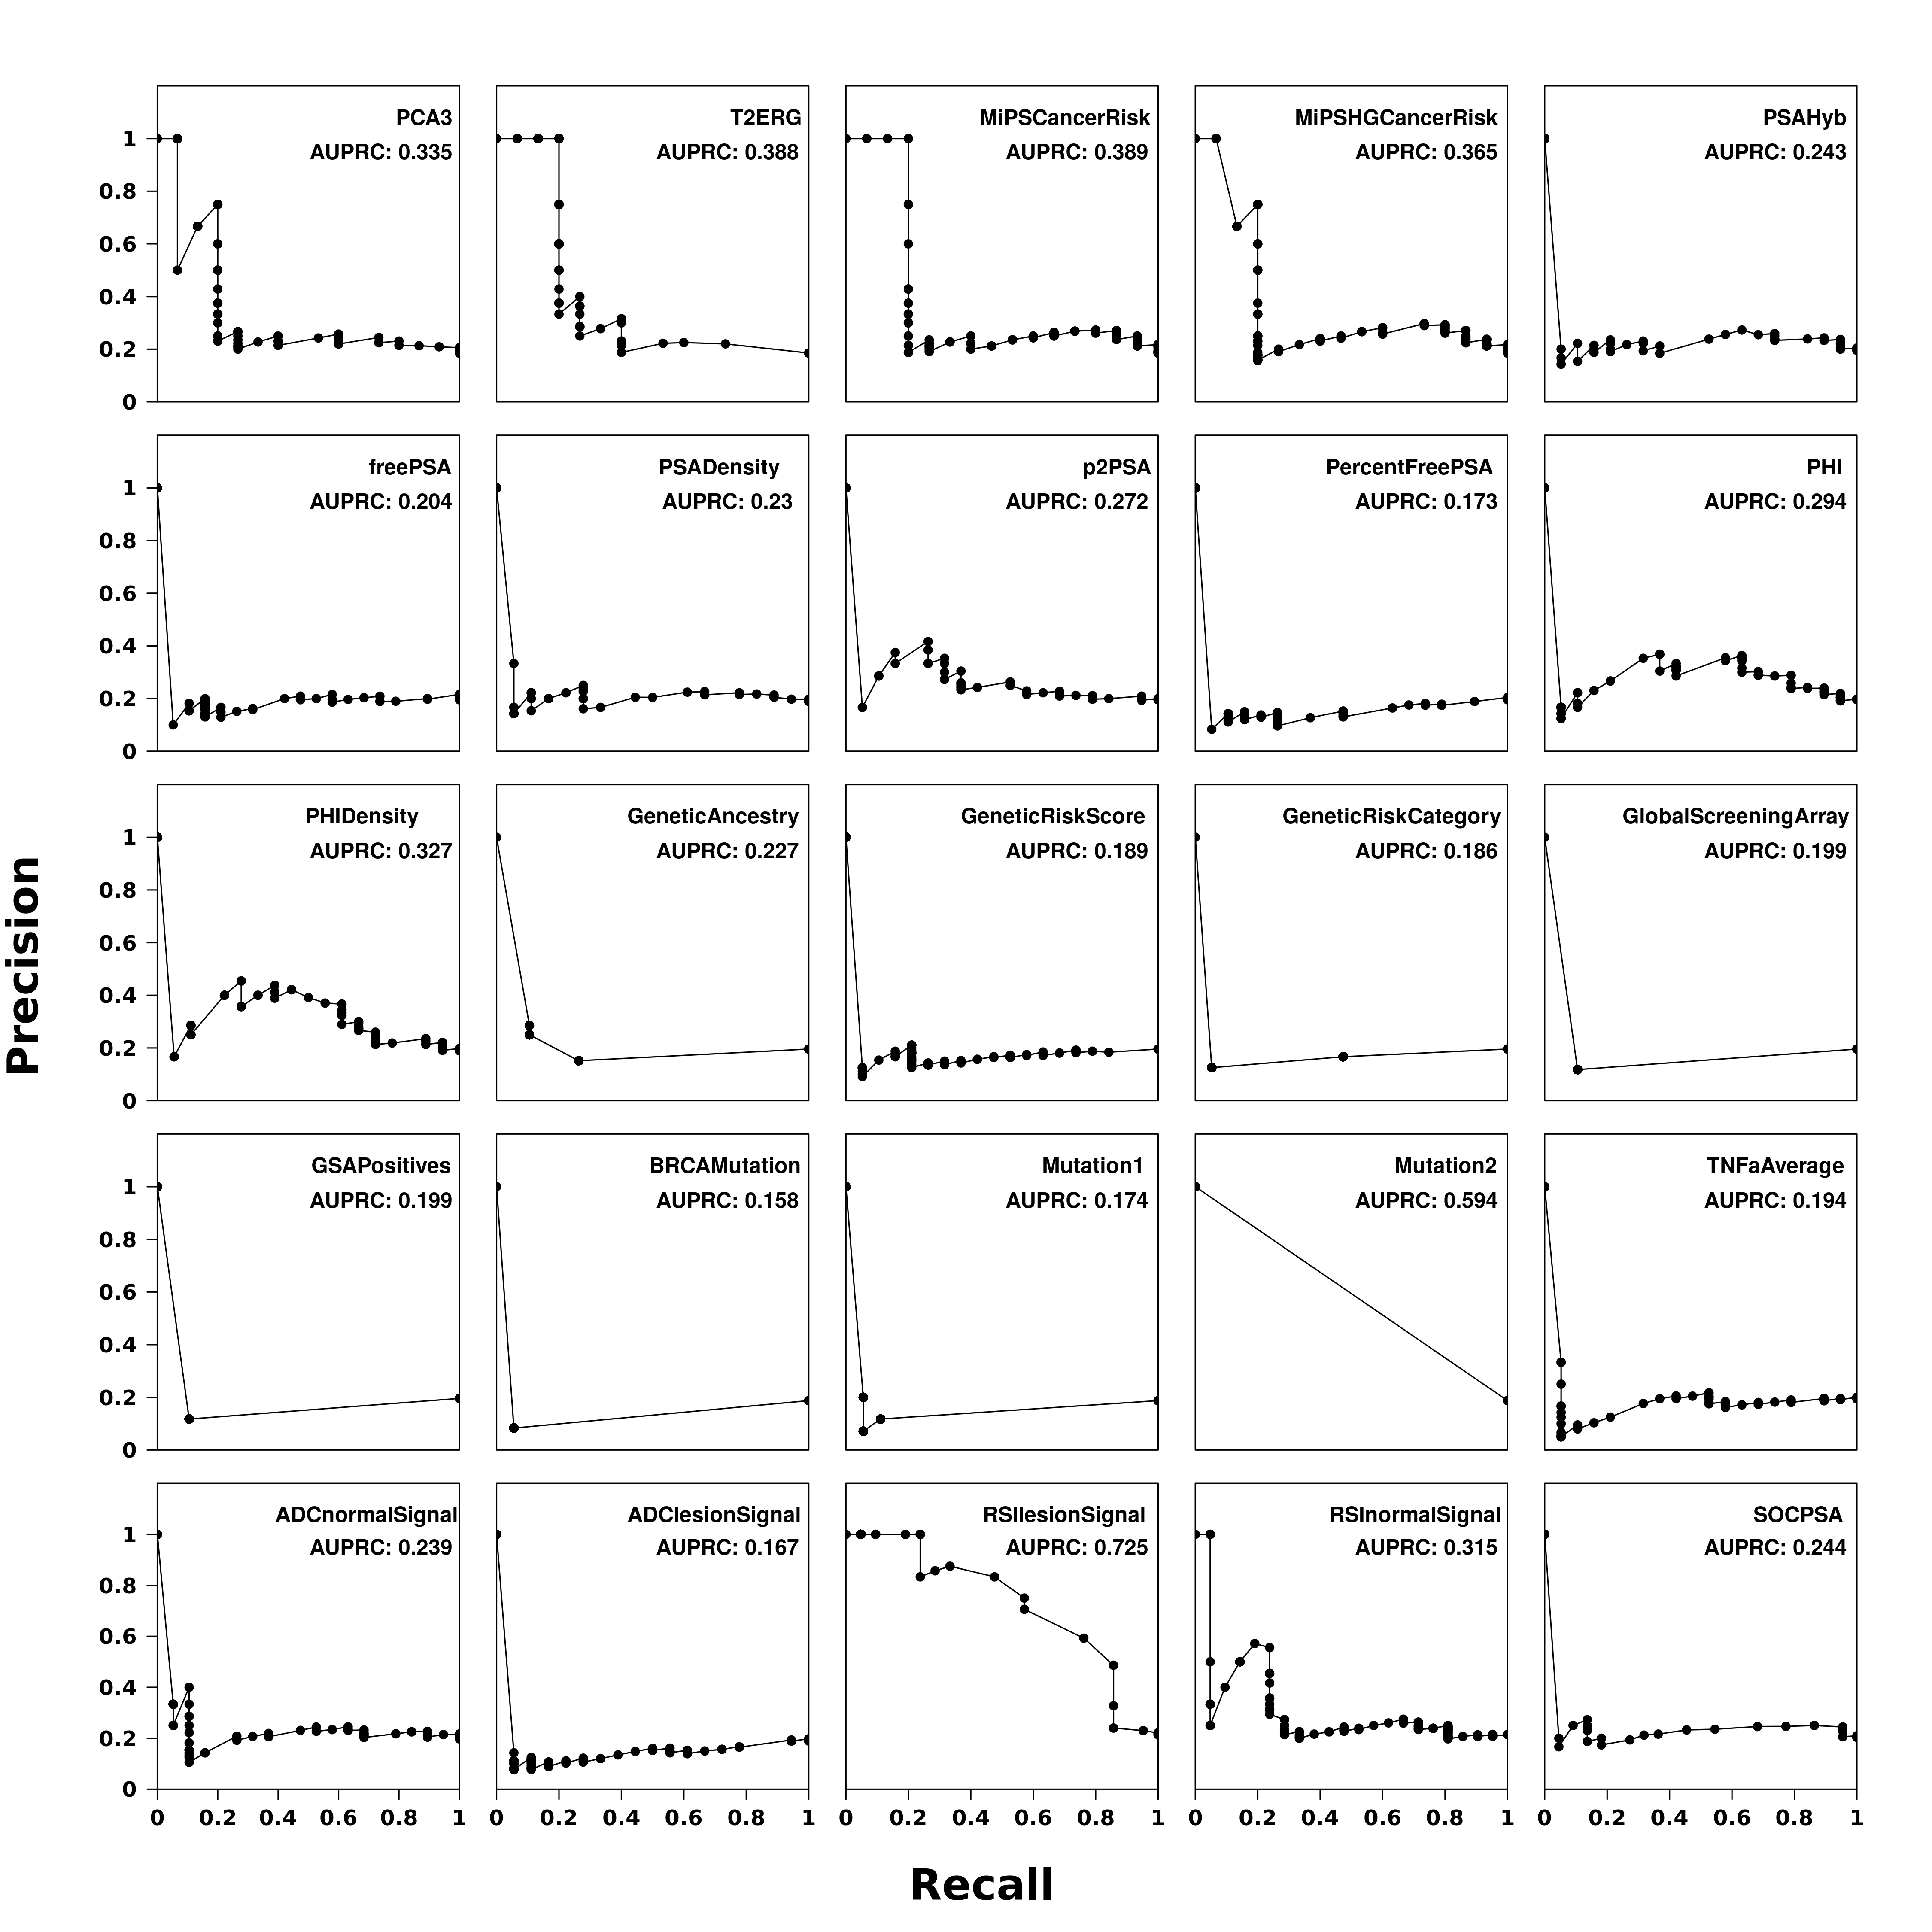
\includegraphics[width=150mm]{png/multipanelplot_prc.png} \\
\caption{Precision-Recall Curves of the tests used in AS.}
\label{fig:PRcurve}
\end{figure}

\noindent We can point out from the figure that the tests in general have low precision, except RSIlesionSignal where particularly shows 
a larger area under the curve in comparison to other tests. The area under the precision-recall curve for each test was 
calculated using the trapezoid rule and its confidence interval was determined. The forest plot for the AUPRC and their 
confidence intervals are shown in Figure~\ref{fig:auprc_plot}. \\
  
\begin{figure}
\centering
    \includegraphics[width=100mm]{png/aupr_plot.png} \\
\caption{Precision-Recall Curves of the tests used in AS.}
\label{fig:auprc_plot}
\end{figure}

\noindent Another plot to look is the ROC curve for each test. It is shown in Figure~\ref{fig:roc_plot}. We can observe that several tests
are on the straight line or even below. That indicates those tests may not have high predictive power. \\

\begin{figure}
\centering
    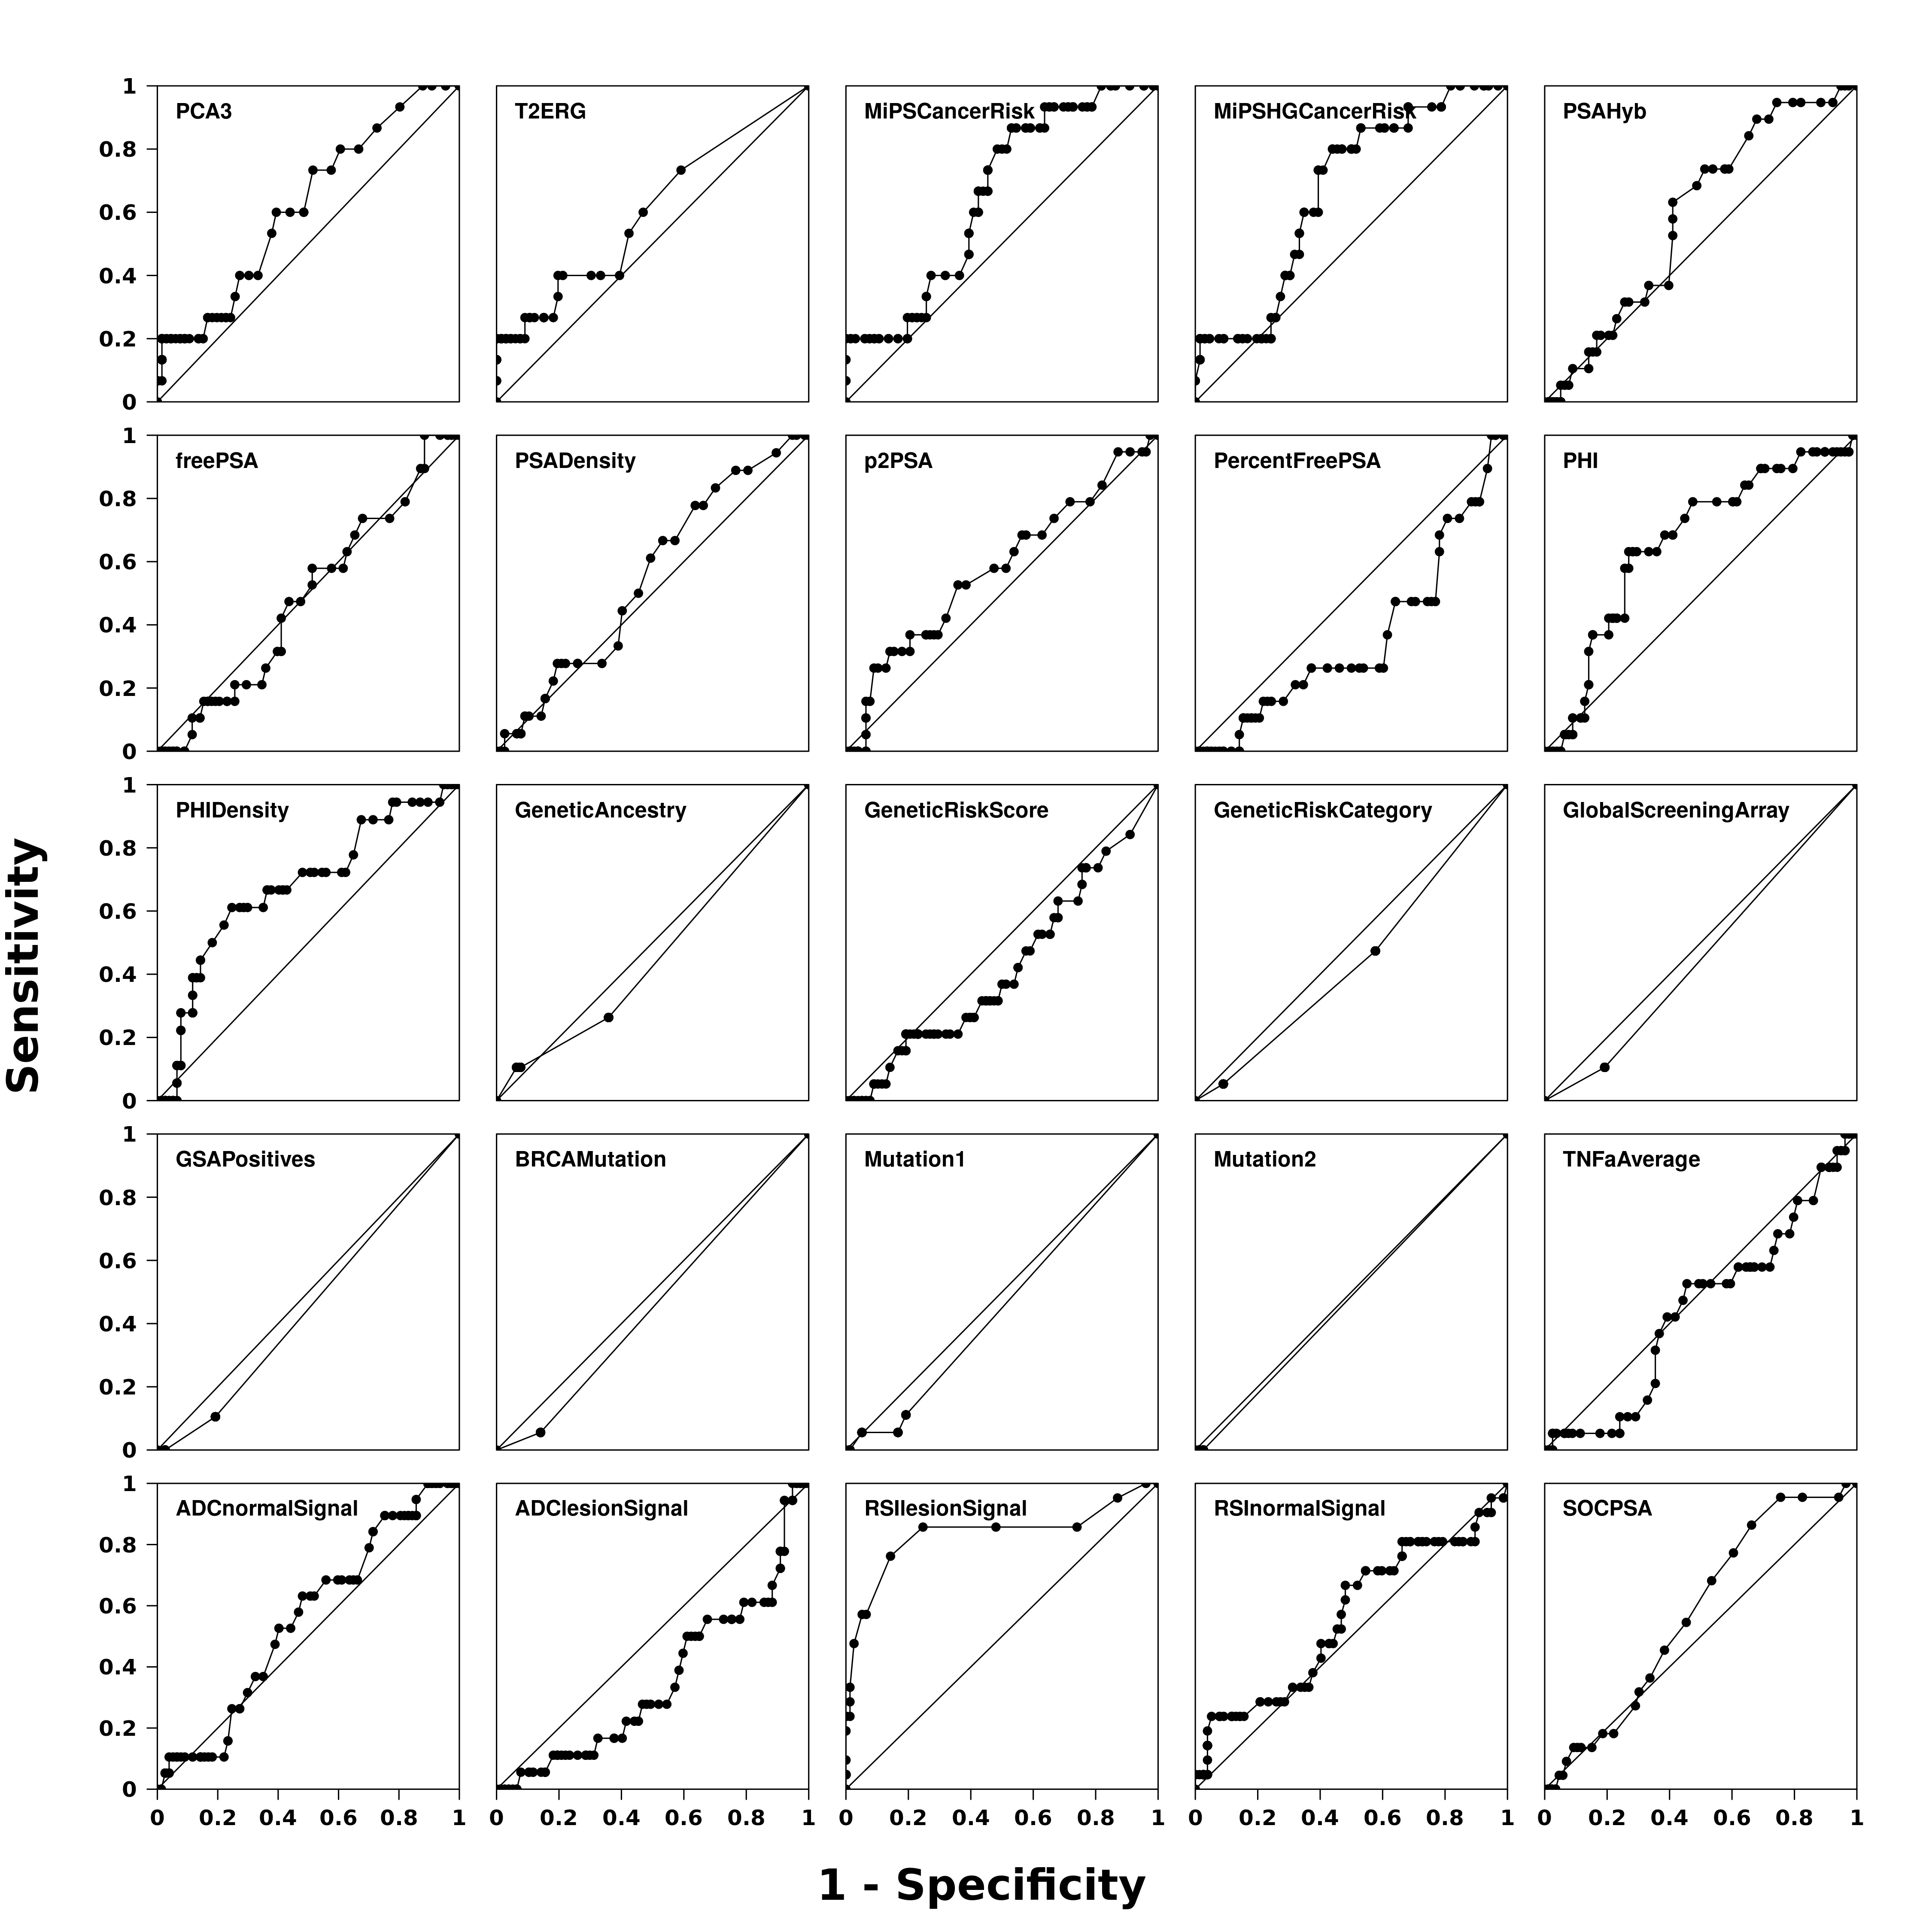
\includegraphics[width=140mm]{png/multipanelploprt_roc.png} \\
\caption{Precision-Recall Curves of the tests used in AS.}
\label{fig:roc_plot}
\end{figure}

\noindent For each test, we save the confusion matrix data for each threshold considered here. In Figure~\ref{fig:specificity},
we plot the specificity of each test against the threshold used.  Thresholds were normalized to simplify the plotting. 
Other plots such as Accuracy and F1 scores are also shown in Figure~\ref{fig:accuracy} and ~\ref{fig:f1}. \\

\begin{figure}
\centering
    \includegraphics[width=150mm]{png/multipanelplot_hexbin_specificity.png} \\
\caption{Specificity of each test against the threshold used.  Thresholds were normalized using the largest value of the test.}
\label{fig:specificity}
\end{figure}

\begin{figure}
\centering
    \includegraphics[width=150mm]{png/multipanelplot_hexbin_accuracy.png} \\
\caption{Accuracy of each test against the threshold used.  Thresholds were normalized using the largest value of the test.}
\label{fig:accuracy}
\end{figure}

%\begin{figure}
%\centering
%    \includegraphics[width=150mm]{png/multipanelplot_hexbin_f1.png} \\
%\caption{F1 scores of each test against the threshold used.  Thresholds were normalized using the largest value of the test.}
%\label{fig:f1}
%\end{figure}

%\noindent Plotting all the tests together in the precision-recall plot is shown in Figure~\ref{fig:alltest}. 

%\begin{figure}
%\centering
%    \includegraphics[width=150mm]{png/all_test.png} 
%\caption{Precision-Recall Plots for the tests considered in this study}
%\label{fig:alltest}
%\end{figure}

\section{Next Steps}
\noindent Perform the analysis with all tests together. Select the operating point that maximizes F1 or sensitivity at 95\%
sensitivity. \\  

%BiopsyResult, BiopsyUpgraded, Observation (False Positive, True Positive, etc), and RSI lesion data is reported in the 
%data.  Since we try to predict aggressiveness, we can group patients by outcome ( FP, TP, TN and FN) and see how those tests 
%did for each of these observations. 

%\noindent The biomarkers used in this study are classified in groups: Urine, Blood/Urine, Blood, Genetics, and 
%Imaging. Establish a relation of these biomarkers with the individuals. What can we say about the results of these 
%tests when race, weight or any other factor is included?


\section{Appendix}

\noindent Current spreadsheet (04/20/2020) has the following columns: \\


\begin{longtable}{| p{.40\textwidth} | p{.60\textwidth} |} 
\hline
{\bf Column Name} & {\bf Description}  \\
  \hline
  Record.ID                 &  A Subject ID number \\
  \hline   
  Age                       &  Age at time of enrollment \\
  \hline
  Race                      &  Race reported by subject \\
  \hline
  Ethnicity                 &  Non-Hispanic or Hispanic  \\
  \hline  
  Weight                    &  Kilograms \\ 
  \hline  
  Height                    &   \Centimeters\
  \hline  
  BMI                       &   \\
  \hline  
  SOCPSA                    &   \\
  \hline
  MRIResult                 &   \\
  \hline
  MRILesions                &   \\
  \hline
  HighestPIRADS             &   \\
  \hline
  BiopsyResult              &   \\
  \hline
  ProstateVolume            &   \\
  \hline
  PreviousGleason           &   \\
  \hline
  PreviousISUP              &   \\
  \hline
  StudyHighestGleason       &   \\
  \hline
  StudyHighestISUP          &   \\
  \hline
  Observation               &   \\
  \hline
  BiopsyUpgraded            &   \\
  \hline
  PCA3                      &   \\
  \hline
  T2ERG                     &   \\
  \hline
  MiPSCancerRisk            &   \\
  \hline
  MiPSHighGradeCancerRisk   &   \\
  \hline
  PSAHyb                    &   \\
  \hline
  freePSA                   &   \\
  \hline
  p2PSA                     &   \\
  \hline
  PercentFreePSA            &   \\
  \hline
  PHI                       &   \\
  \hline
  GeneticAncestry           &   \\
  \hline
  GeneticRiskScore          &   \\
  \hline
  GeneticRiskCategory       &   \\
  \hline
  GlobalScreeningArray      &   \\
  \hline
  GSAPositives              &   \\
  \hline
  BRCAMutation              &   \\
  \hline
  Mutation1                 &   \\   
  \hline
  Mutation.2                &   \\ 
  \hline
  TNFaAverage               &   \\   
  \hline
  TNFaSTD                   &   \\ 
  \hline
  RSInormalSignal           &   \\   
  \hline
  RSIlesionSignal           &   \\ 
  \hline
  ADCnormalSignal           &   \\   
  \hline
  ADClesionSignal           &   \\ 
  \hline
  RSIlesionPIRADS           &   \\   
  \hline
  RSIlesionCancer           &   \\ 
  \hline
  RSIlesionGleason          &   \\   
  \hline
  RSIlesionISUP             &   \\ 
  \hline
  RSIlesionUpgraded         &   \\   
  \hline
  RSIlesionObservation      &   \\ 
  \hline
  ProgressedToTreatment     &   \\   
  \hline
  Prostatectomy             &   \\ 
  \hline
  UpgradedAndProgressed     &   \\   
  \hline
  NoUpgradeAndProgressed    &   \\ 
  \hline
  DaysBxToProgression       &   \\   
  \hline
  DaysBxToLastClinicalAppt  &   \\ 
  \hline
  DaysBxToLastReview        &   \\   
  \hline
  DaysDxToUpgrade           &   \\ 
  \hline
  DaysDxToProgression       &   \\   
  \hline
  DaysDxToLastClinicalAppt  &   \\ 
  \hline
  DaysDxToLastReview        &   \\ 
  \hline



% BiopsyUpgraded           &    Research study biopsy increased cancer grade from most recent previous biopsy result
% PCA3                     &    Urinary biomarker
% T2ERG                    &    Urinary biomarker
% MiPSCancerRisk           &    Urinary/Blood biomarker using PSA, PCA3, T2ERG (Mi-Prostate Score Cancer Risk)
% MiPSHighGradeCancerRisk  &    Urinary/Blood biomarker using PSA, PCA3, T2ERG (Mi-Prostate Score High Grade Cancer Risk, Gleason Score ≥7)
% PSAHyb                   &    Blood biomarker (Access Hybritech PSA assay)
% freePSA                  &    Blood biomarker (amount of unbound PSA)
% p2PSA                    &    Blood biomarker ([-2]proPSA, precursor of PSA)
% PercentFreePSA           &    Blood biomarker (percentage of unbound PSA)
% PHI                      &    Blood biomarker (Prostate Health Index)
% GeneticAncestry          &    Genetic biomarker
% GeneticRiskScore         &    Genetic biomarker
% GeneticRiskCategory      &    Genetic biomarker (Genetic risk rating, low, normal, high)
% GlobalScreeningArray     &    Genetic biomarker (Global Screening Array positive or negative for gene mutation)
% GSAPositives             &    Genetic biomarker (Global Screening Array number of positive gene mutations)
% BRCAMutation             &    Genetic biomarker (BRCA1 or BRCA2 gene mutation)
% Mutation1                &    Genetic biomarker (Global Screening Array gene mutation name/type)
% Mutation 2               &    Genetic biomarker (Global Screening Array gene mutation name/type)
% RSInormalSignal          &    Imaging biomarker (Resticted Spectrum Imaging value on location of normal tissue noted on MRI)
% RSIlesionSignal          &    Imaging biomarker (Resticted Spectrum Imaging value on location of lesion tissue noted on MRI)
% ADCnormalSignal          &    Imaging biomarker (Apparent Diffusion Coefficient value on location of normal tissue noted on MRI, current use for prostate lesion rating)
% ADClesionSignal          &    Imaging biomarker (Apparent Diffusion Coefficient value on location of lesion tissue noted on MRI, current use for prostate lesion rating)




\caption{Your caption here} % needs to go inside longtable environment
\label{tab:myfirstlongtable}
\end{longtable}





\begin{thebibliography}{}
\bibitem{JAMES}
  James, G.~{\textit{et al.}}. An Introduction to Statistical Learning. Springer. 7th Printing.
\bibitem{BPG}
C.~P'ng.~{\textit{et al.}}. BPG: Seamless, Automated and Interactive Visualization of Scientific Data.
\textit{BMC Bioinformatics} 20, 42 (2019).\\

\end{thebibliography}


\end{document}

% Record ID                &    Subject ID number
% Age                      &    Age at time of enrollment
% Race                     &    Reported by subject
% Ethnicity                &    Non-Hispanic or Hispanic
% Weight                   &    Kilograms
% Height                   &    Centimeters
% BMI                      &    Body Mass Index (BMI)
% MRIResult                &    Prostate MRI positive or negative for lesions per radiologist  (0 : Negative , 1: Positive)
% MRILesions               &    Number of MRI lesions of MRI was positive (0 or 1)
% HighestPIRADS            &    Risk rating by radiologist of any lesions found on prostate MRI (rating 1-5, 0 signifies no lesion found)
% BiopsyResult             &    Prostate cancer confirmed via biopsy
% ProstateVolume           &    Cubic centimeters
% PreviousGleason          &    Most recent prostate cancer Gleason score rating prior to research biopsy (rating X+X, primary and secondary rating)
% PreviousISUP             &    Most recent prostate cancer International Society of Urological Pathologists score rating prior to research biopsy (rating 1-5)
% StudyHighestGleason      &    Prostate cancer Gleason score rating during research study after research MRI (rating X+X, primary and secondary rating)
% StudyHighestISUP         &    Prostate cancer International Society of Urological Pathologists score rating during research study after research MRI (rating 1-5)
% Observation              &    Results of research MRI compared to research biopsy
% BiopsyUpgraded           &    Research study biopsy increased cancer grade from most recent previous biopsy result
% PCA3                     &    Urinary biomarker
% T2ERG                    &    Urinary biomarker
% MiPSCancerRisk           &    Urinary/Blood biomarker using PSA, PCA3, T2ERG (Mi-Prostate Score Cancer Risk)
% MiPSHighGradeCancerRisk  &    Urinary/Blood biomarker using PSA, PCA3, T2ERG (Mi-Prostate Score High Grade Cancer Risk, Gleason Score ≥7)
% PSAHyb                   &    Blood biomarker (Access Hybritech PSA assay)
% freePSA                  &    Blood biomarker (amount of unbound PSA)
% p2PSA                    &    Blood biomarker ([-2]proPSA, precursor of PSA)
% PercentFreePSA           &    Blood biomarker (percentage of unbound PSA)
% PHI                      &    Blood biomarker (Prostate Health Index)
% GeneticAncestry          &    Genetic biomarker
% GeneticRiskScore         &    Genetic biomarker
% GeneticRiskCategory      &    Genetic biomarker (Genetic risk rating, low, normal, high)
% GlobalScreeningArray     &    Genetic biomarker (Global Screening Array positive or negative for gene mutation)
% GSAPositives             &    Genetic biomarker (Global Screening Array number of positive gene mutations)
% BRCAMutation             &    Genetic biomarker (BRCA1 or BRCA2 gene mutation)
% Mutation1                &    Genetic biomarker (Global Screening Array gene mutation name/type)
% Mutation 2               &    Genetic biomarker (Global Screening Array gene mutation name/type)
% RSInormalSignal          &    Imaging biomarker (Resticted Spectrum Imaging value on location of normal tissue noted on MRI)
% RSIlesionSignal          &    Imaging biomarker (Resticted Spectrum Imaging value on location of lesion tissue noted on MRI)
% ADCnormalSignal          &    Imaging biomarker (Apparent Diffusion Coefficient value on location of normal tissue noted on MRI, current use for prostate lesion rating)
% ADClesionSignal          &    Imaging biomarker (Apparent Diffusion Coefficient value on location of lesion tissue noted on MRI, current use for prostate lesion rating)
% RSIlesionPIRADS          &    Risk rating by radiologist of any lesions found in location of RSI value on prostate MRI (rating 1-5, 0 signifies no lesion found)
% RSIlesionCancer          &    Prostate cancer confirmed via biopsy in location of RSI value
% RSIlesionGleason         &    Prostate cancer Gleason score rating in location of RSI value (rating X+X, primary and secondary rating)
% RSIlesionISUP            &    Prostate cancer International Society of Urological Pathologists score rating in location of RSI value (rating 1-5)
% RSIlesionUpgraded        &    Increased cancer grade from most recent previous biopsy result in location of RSI value
% RSIlesionObservation     &    Results of research MRI compared to research biopsy in location of RSI value
